\documentclass[english]{article}
\usepackage[T1]{fontenc}
\usepackage[utf8]{inputenc}
%\usepackage[latin9]{inputenc}
\usepackage{geometry}
\usepackage{cite}
\usepackage[english]{babel}
\usepackage{graphicx}
\usepackage{framed}
\usepackage[normalem]{ulem}
\usepackage{amsmath}
\usepackage{amsthm}
\usepackage{amssymb}
\usepackage{amsfonts}
\usepackage{enumerate}
\usepackage{algorithm}  
\usepackage{algorithmicx}  
\usepackage{algpseudocode} 
\usepackage[utf8]{inputenc}
\usepackage[UTF8]{ctex}
\geometry{verbose,tmargin=3cm,bmargin=2cm,lmargin=3cm,rmargin=3cm}
%\usepackage[top=1 in,bottom=1in, left=1 in, right=1 in]{geometry}
\usepackage{float}

%A bunch of definitions that make my life easier
\newcommand{\matlab}{{\sc Matlab} }
\newcommand{\cvec}[1]{{\mathbf #1}}
\newcommand{\rvec}[1]{\vec{\mathbf #1}}
\newcommand{\ihat}{\hat{\textbf{\i}}}
\newcommand{\jhat}{\hat{\textbf{\j}}}
\newcommand{\khat}{\hat{\textbf{k}}}
\newcommand{\minor}{{\rm minor}}
\newcommand{\trace}{{\rm trace}}
\newcommand{\spn}{{\rm Span}}
\newcommand{\rem}{{\rm rem}}
\newcommand{\ran}{{\rm range}}
\newcommand{\range}{{\rm range}}
\newcommand{\mdiv}{{\rm div}}
\newcommand{\proj}{{\rm proj}}
\newcommand{\R}{\mathbb{R}}
\newcommand{\N}{\mathbb{N}}
\newcommand{\Q}{\mathbb{Q}}
\newcommand{\Z}{\mathbb{Z}}
\newcommand{\<}{\langle}
\renewcommand{\>}{\rangle}
\renewcommand{\emptyset}{\varnothing}
\newcommand{\attn}[1]{\textbf{#1}}
\theoremstyle{definition}
\newtheorem{theorem}{Theorem}
\newtheorem{corollary}{Corollary}
\newtheorem*{definition}{Definition}
\newtheorem*{example}{Example}
\newtheorem*{note}{Note}
\newtheorem{exercise}{Exercise}
\newcommand{\bproof}{\bigskip {\bf Proof. }}
\newcommand{\eproof}{\hfill\qedsymbol}
\newcommand{\Disp}{\displaystyle}
\newcommand{\qe}{\hfill\(\bigtriangledown\)}
\setlength{\columnseprule}{1 pt}
\renewcommand{\algorithmicrequire}{\textbf{Input:}}  % Use Input in the format of Algorithm  
\renewcommand{\algorithmicensure}{\textbf{Output:}} % Use Output in the format of Algorithm
\usepackage{babel}
\begin{document}
\title{Face Recognition with Tensor SVD}
\author{Shanwen Pu,\quad Siya Liu}
\maketitle


\abstract{A tensor is a multidimensional array. First-order tensors and second-order tensors can be viewed as
vectors and matrices, respectively. Traditional tensor algebra generalize matrix SVD to CP decomposition and HOSVD. But in the recently new tensor framework, T-SVD is another generalization of matrix SVD with nearly the same representation. Moreover, the new tensor product(t-product) can be accelerated by FFT, which improves our T-SVD.
We solve the face recognition task on several databases by new robust SVD(TRSVD) and compare our new method with several popular methods, e.g PCA, Tensor QR to verify performance and stability.}

\section{Introduction}
To develop automatic procedures for face recognition that are robust with respect to varying conditions is a challenging research problem. PCA(SVD) is a popular technique, but it doesn't perform well when several environment factors are varied. By letting the modes of the tensor represent a different viewing condition, it became possible to improve the precision of the recognition algorithm compared to PCA.\\

A tensor is a multidimensional array. A first-order tensor is a vector, a second-order tensor is a matrix, and a tensor of order 3 or higher is a higher order tensor. In many cases, it is appropriate to store data in higher-order multidimensional arrays, such as storing photos and videos. As a result, a number of tensor decompositions, such as CANDECOMP/PARAFAC(CP), Tucker, and higher-order SVD and tensor-tensor decomposition, have been developed to facilitate the extension of linear algebra tools to this multilinear context.\\

Instead of considering images as vetorized objects (in traditional matrix-based PCA and in TensorFaces), the approach we use here is based on T-SVD, which is presented in \cite{hao2013facial}. This method has an advantage over TensorFaces(based on HOSVD) in that it does not require a least square solve for the coeffcients. Moreover, we will use a pivoted tensor QR decomposition as an alternative tensor decomposition scheme with a potential advantage in updating and downdating the original image data.
\section{Related Work}
Face recognition task can be tackled by several classes of methods, among which matrix or tensor decomposition based method is of our interest. 
\paragraph{PCA based methods}
PCA was invented in 1901 by Karl Pearson\cite{pearson1901liii}, and
it has since been a classical technique in image recognition and compression. In simple terms,
PCA is used to transform a number of possibly correlated variables into a smaller number of
uncorrelated variables known as principal components. The first few principal components
explain most of the variation in the original data, while the remaining ones make a negligible
contribution. Thus we can describe the data more economically using the first several principal
components. 
\paragraph{Traditional tensor decomposition based methods}
TensorFaces \cite{vasilescu2002multilinear} was the first algorithm to handle the facial recognition
problem by manipulating tensors. In this algorithm, the data is represented as a tensor
with different modes for different factors. One way in which the algorithm is consistent with
traditional PCA is that the images are still vectorized. The multidimensionality therefore is
obtained only by using the other modes to represent other features of the data. The approximation
of the tensor is done by use of the multidimensional higher-order SVD (HOSVD),
which is a Tucker type of representation. 
\paragraph{New tensor framework and T-SVD based methods}
T-SVD is a new approach invented by Kilmer, etc \cite{kilmer2008third}\cite{kilmer2011factorization}\cite{kilmer2013third} as another generalization of matrix SVD, by brand new tensor framework\cite{kilmer2011factorization} . T-SVD representation coincides with matrix SVD and the tensor-tensor product in new framework can be accelerated by fast Fourier transform, which will improve the performance of this method. T-SVD method I and II by hao \cite{hao2013facial} is based on new T-SVD and T-SVD II adopt the new SVD in Fourier domain, which has the potential for further compression of the information in the database. 
\paragraph{Robust PCA and t-SVD} Tensor Robust Principal Component (TRPCA)\cite{lu2016tensor} problem which extends the known Robust PCA \cite{candes2011robust} to the tensor case. TRPCA is a new tensor Singular Value Decomposition (t-SVD) \cite{kilmer2011factorization} and its induced tensor tubal rank and tensor nuclear norm. Interestingly, TRPCA involves RPCA as a special case when 3rd-order $n_3 = 1$ and thus it is a simple and elegant tensor extension of RPCA. Also numerical experiments verify our theory and the application for the image denoising demonstrates the effectiveness of our method. 

\section{Your algorithm/model/approach}
T-SVD: analogous to the matrix SVD, is a generalization of matrix multiplication for tensors of order three.\\
Let $ \mathcal A $ be an $ l\times m \times n $ real-valued tensor; then $ \mathcal A $ can be factored as 
$$ \mathcal A=\mathcal U*\mathcal S*\mathcal V^{T} $$
with an $ l\times m \times n $ orthogonal tensor $ \mathcal U $, an $ m\times m \times n $ orthogonal tensor $ \mathcal V $, and an $ l\times m \times n $ f-diagonal tensor $ \mathcal S $.\\
The multiplication is based on a convolution-like operation, which can be implemented efficiently using the Fast Fourier Transform.\\
Robust T-SVD: extends T-SVD to robust T-SVD.\\
Consider that we have a 3-way tensor $ \mathcal X $ such that $ \mathcal X=\mathcal L_{0}+\mathcal S_{0} $, where $ \mathcal L_0 $ has low tubal rank and $ \mathcal S_0 $ is sparse. We can recover both the low-rank and the sparse components exactly by simply solving a convex program whose objective is a weighted combination of the tensor nuclear norm and the $l_1$-norm, i.e
$$ \min ||\mathcal L ||_{*}+\lambda||\mathcal E||_{1}, \ s.t. \mathcal X=\mathcal L+\mathcal E $$

\section{Tensor Algebra}
\paragraph{Order of tensor} The order of a tensor is the dimensionality of the array needed to represent it, also known as ways or modes. 
An order-p  tensor  $\mathcal{A}$  is a  p-dimensional array. It can be written as
$$\mathcal{A}=\left(a_{i_{1} i_{2} \ldots i_{p}}\right) \in \mathbb{R}^{n_{1} \times n_{2} \times \cdots \times n_{p}}$$
\paragraph{Tensor-Matrix Multiplication} An important operation for a tensor is the tensor-matrix multiplication, also known as mode-n product. Given a tensor $ \mathcal{A} \in \mathbb{R}^{d_{1} \times d_{2} \times \cdots \times d_{N}} $ and a matrix $ M \in   \mathbb{R}^{c_{n}} \times d_{n}$,  the mode-  $n $ product is a tensor
$$ \mathcal{B}=\mathcal{A} \times_{n} M \in \mathbb{R}^{d_{1} \times \cdots \times d_{n-1} \times c_{n} \times d_{n+1} \cdots \times d_{N}} $$
where $$
b_{i_{1}, \ldots, i_{n-1}, j_{n}, i_{n+1}, \ldots, i_{N}}:=\sum_{i_{n}=1}^{d_{n}} a_{i_{1}, \ldots, i_{n-1}, i_{n}, i_{n+1}, \ldots, i_{N}} m_{j_{n}, i_{n}} $$
for $ j_{n}=1,2, \ldots, c_{n} $.
\paragraph{Tensor Decompositions} A decomposition of a tensor $ \mathcal{A} \in \mathbb{R}^{d_{1} \times d_{2} \times \cdots \times d_{N}} $ is of the form
$$
\mathcal{A}=\mathcal{B} \times_{1} S^{(1)} \times_{2} S^{(2)} \times \cdots \times_{N} S^{(N)} $$
where $ \mathcal{B} \in \mathbb{R}^{c_{1} \times c_{2} \times \cdots \times c_{N}} $ is called the core tensor, and $ S^{(n)} \in \mathbb{R}^{d_{n} \times c_{n}} $ for $ n=1, \ldots, N $ are called side-matrices. An illustration is given in Figure 1.
\begin{figure}[!h]
	\centering
	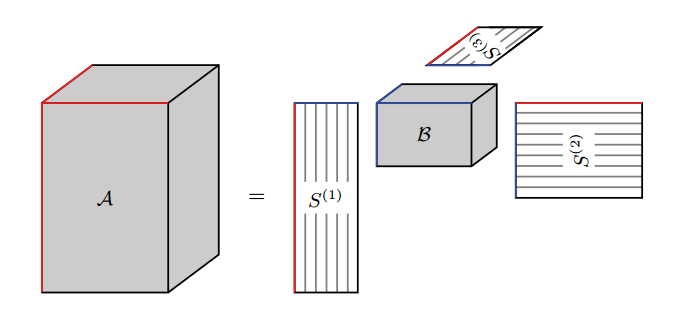
\includegraphics[scale=0.6]{decomposition}
	\caption{Tensor Decompositions}
\end{figure}
\paragraph{Fold and Unfold Operators} We make use of the fold and unfold operators. Suppose that  $\mathcal{A} \in \mathbb{R}^{n_{1} \times n_{2} \times n_{3}}$ and that each frontal face of the tensor is defined by  $n_{1} \times n_{2}$  matrices  $\mathcal{A}(:,:, 1), \ldots,   \mathcal{A}\left(:,:, n_{3}\right)$.  Then unfold is defined by
\begin{equation*}
\operatorname{unfold}(\mathcal{A}, 1)=\left[\begin{array}{c}
\mathcal{A}(:,:, 1) \\
\mathcal{A}(:,:, 2) \\
\vdots \\
\mathcal{A}\left(:,:, n_{3}\right)
\end{array}\right] \in \mathbb{R}^{n_{1} n_{3} \times n_{2}}
\end{equation*}
The second argument of unfold specifies which orientation of the tensor to unfold (see Figure 1.2 ). For example, $unfold  (\mathcal{A}, 1)$  unstacks the tensor according to its front-back faces. Similarly, $unfold(  \mathcal{A}, 2  )$ refers to unstacking by faces defined by slicing the tensor side to side and $unfold  (\mathcal{A}, 3)$  unstacks by slicing top to bottom. See Figure 3.1 for an example.
\paragraph{Block-Circulant Matrix} It is possible to create a block-circulant matrix from the slices of a tensor. For example, if  $\mathcal{A} \in \mathbb{R}^{n_{1} \times n_{2} \times n_{3}}$  with  $n_{1} \times n_{2}$  frontal faces  $A_{1}=\mathcal{A}(:,:, 1), \ldots, A_{n_{3}}=\mathcal{A}( 
\left.; n_{3}\right)$  then
\begin{equation*}
\operatorname{bcirc}(\operatorname{unfold}(\mathcal{A}, 1))=\left[\begin{array}{ccccc}
A_{1} & A_{n_{3}} & A_{n_{3}-1} & \dots & A_{2} \\
A_{2} & A_{1} & A_{n_{3}} & \dots & A_{3} \\
\vdots & \ddots & \ddots & \ddots & \vdots \\
A_{n_{3}} & A_{n_{3}-1} & \ddots & A_{2} & A_{1}
\end{array}\right]
\end{equation*}
\paragraph{Tensor Product} Let  $\mathcal{A}$  be  $n_{1} \times n_{2} \times n_{3}$  and  $\mathcal{B}$  be  $n_{2} \times \ell \times n_{3}$ .  Then the product
$\mathcal{A} * \mathcal{B}$  is the  $n_{1} \times \ell \times n_{3}$  tensor
$$\mathcal{A} * \mathcal{B}=\text { fold }(\operatorname{circ}(\text { unfold }(\mathcal{A}, 1)) \cdot \operatorname{unfold}(\mathcal{B}, 1), 1)$$
\text { LEMMA1 }  $$\mathcal{A} *(\mathcal{B} * \mathcal{C})=(\mathcal{A} * \mathcal{B}) * \mathcal{C}$$
\text { LEMMA2 }
$$\left.\left(\mathcal{A}^{T} * \mathcal{B}\right)(1: k,:, ;)=(\mathcal{A}(:, 1: k,:))^{T} * \mathcal{B}\right)$$
\paragraph{Identity Tensor} The  $n \times n \times \ell$  identity tensor  $\mathcal{I}_{n n \ell}$  is the tensor whose front face is the  $n \times n$  identity matrix, and whose other faces are all zeros.
\paragraph{Inverse Tensor} An  $n \times n \times n$  tensor  $\mathcal{A}$  has an inverse  $\mathcal{B}$  provided that
$$\mathcal{A} * \mathcal{B}=\mathcal{I}, \quad \text { and } \quad \mathcal{B} * \mathcal{A}=\mathcal{I}$$
\paragraph{Tensor Transpose} If  $\mathcal{A}$  is  $n_{1} \times n_{2} \times n_{3}$,  then  $\mathcal{A}^{T}$  is the $ n_{2} \times n_{1} \times n_{3}$  tensor obtained by transposing each of the front-back faces and then reversing the order of transposed faces 2 through  $n_{3}$ . In other words,
$$\mathcal{A}^{T}=\text { fold }\left(\text { unfold }\left(\mathcal{A}, 1,\left[1, n_{3}:-1: 2\right]\right), 1\right)$$
\text { LEMMA3 }   Suppose  $\mathcal{A}, \mathcal{B}$  are two tensors such that  $\mathcal{A} * \mathcal{B}$  and  $\mathcal{B}^{T} * \mathcal{A}^{T}$  is defined. Then  $(\mathcal{A} * \mathcal{B})^{T}=\mathcal{B}^{T} * \mathcal{A}^{T}$.
\paragraph{Orthogonal Tensor} An $ n \times n \times \ell $ real-valued tensor $ \mathcal{Q} $ is orthogonal if $ \mathcal{Q}^{T} * \mathcal{Q}= \mathcal{Q} * \mathcal{Q}^{T}=\mathcal{I}$.
\paragraph{Permutation Tensor} A permutation tensor is an $ n \times n \times \ell $ tensor  $\mathcal{P}=\left(p_{i j k}\right)$  with exactly $ n $ entries of unity, such that if  $p_{i j k}=1$,  it is the only non-zero entry in row i, column j, and slice k.
\paragraph{F-Norm of Tensor} Suppose $\mathcal{A}=\left(a_{i j k}\right)$ is size $ n_{1} \times n_{2} \times n_{3} $.  Then
$$ \|\mathcal{A}\|_{F}=\sqrt{\sum_{i=1}^{n_{1}} \sum_{j=1}^{n_{2}} \sum_{k=1}^{n_{3}} a_{i j k}^{2}} $$
\paragraph{Tensor SVD} 
Let A be a $l \times m \times n$ $real-valued$ tensor; 
then A can be factored as 
$$\mathcal{A}=\mathcal{U} * \mathcal{S} * \mathcal{V}^{T}$$
with $\ell \times \ell \times n$ orthogonal tensor $\mathcal{U}$, $m \times m \times n$ orthogonal tensor $\mathcal{V}$, and $\ell \times m \times n$ $f-diagonal$ tensor $\mathcal{S}$. An illustration is given in Figure 2.
\begin{figure}[!h]
	\centering
	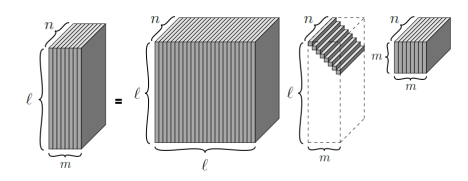
\includegraphics[scale=0.8]{tsvd}
	\caption{Tensor SVD}
\end{figure}
\paragraph{Tensor Pivoted QR Factorization} 
Let A be a $l \times m \times n$ $real-valued$ tensor; 
then A can be factored as 
$$\mathcal{A} * \mathcal{P}=\mathcal{Q} * \mathcal{R}$$
where $\mathcal{Q}$ is an $\ell \times \ell \times n$ orthogonal tensor, $\mathcal{R}$ is an $\ell \times m \times n$ $f-upper$ triangular tensor, and
$\mathcal{P}$ is a permutation tensor.
\section{Algorithms}
% algorithm for pca
\begin{algorithm}  
	\caption{Traditional Matrix PCA Method.}
	\begin{algorithmic} 
		\Require  
		Training:  $\mathbf{I}_{i}$, $i=1,2, \ldots, N; $ Testing: $ \mathbf{J}$;  Truncation index $ k $
		\Ensure  
		Comparison of Test Image with Compressed Training Set  
		\For  {$i=1 \quad to \quad N $}
		\State $ \mathbf{L}(:, i) \leftarrow $ vectorized $ \mathbf{I}_{i} $
		\EndFor
		\State $ \mathbf{M} \leftarrow $ mean image
		\State $ \mathbf{A} \leftarrow $ mean-deviation form of $ \mathbf{L}  $
		\State $ \mathbf{U} \leftarrow $ left singular vectors of $ \mathbf{A} $  
		\State $\mathbf{G} \leftarrow \mathbf{U}(:, 1: k)^{T} \mathbf{A} $
		\State $ \mathbf{T} \leftarrow \mathbf{J}-\mathbf{M} $
		\State $ \mathbf{t} \leftarrow $ vectorized form of $ \mathbf{T} $  
		\State $ \mathbf{c} \leftarrow \mathbf{U}(:, 1: k)^{T} \mathbf{t}  $
		\For  {$j=1 \quad to \quad N $}
		\State do Calculate $ \|c-\mathbf{G}(:, j)\|_{F}$
		\EndFor
		\State Claim that the training image whose coefficient is closest to that of the test image is the match. 
	\end{algorithmic}
\end{algorithm}  

% algorithm for t-svd
\begin{algorithm}  
	\caption{T-SVD Method.}
	\begin{algorithmic} 
		\Require  
		Training:  $\mathbf{I}_{i}$, $i=1,2, \ldots, N, $ Testing: $ \mathbf{J}$,  Truncation index $ k $
		\Ensure  
		Match of Test image against Compressed Representation of Training Set  
		\For  {$i=1 \quad to \quad N $}
		\State  $\mathcal{L}(:, i,:) \leftarrow \mathbf{I}_{i}$
		\EndFor
		\State $ \mathcal{M} \leftarrow $ mean image
		\State $ \mathcal{A} \leftarrow $ mean-deviation form of $ \mathcal{L}  $
		\State $ \mathcal{U} \leftarrow $ left singular vectors of tensor $ \mathcal{A} $
		\State $ \mathcal{C} \leftarrow \mathcal{U}(:, 1: k,:)^{T} * \mathcal{A} $
		\State $ \mathcal{T}(:, 1,:) \leftarrow \operatorname{twist}(\mathbf{J}-\mathcal{M})  $
		\State $ \mathcal{B} \leftarrow \mathcal{U}(:, 1: k,:)^{T} * \mathcal{T} $
		\For  {$j=1 \quad to \quad N $}
		\State Calculate $ \|\mathcal{B}-\mathcal{C}(:, j,:)\|_{F} $
		\EndFor
		\State Claim that the training image whose coefficient is closest to that of the test image is the match. 
	\end{algorithmic}
\end{algorithm}

% algorithm for tqr
\begin{algorithm}  
	\caption{Tensor QR Method.}
	\begin{algorithmic} 
		\Require  
		Training:  $\mathbf{I}_{i}$, $i=1,2, \ldots, N; $ Testing: $ \mathbf{J}$,  Truncation index $ k $
		\Ensure  
		Coefficients of testing images with a basis of reduced dimension  
		\For  {$i=1 \quad to \quad N $}
		\State  $\mathcal{L}(:, i,:) \leftarrow \mathbf{I}_{i}$
		\EndFor
		\State $ \mathcal{M} \leftarrow $ mean image
		\State $ \mathcal{A} \leftarrow $ mean-deviation form of $ \mathcal{L}  $
		\State $ [Q, \mathcal{R}] \leftarrow $ tensor (pivoted) QR decomposition of $ \mathcal{A}  $
		\State $ \mathcal{C} \leftarrow \mathcal{Q}(:, 1: k,:)^{T} * \mathcal{A} $
		\State $ \mathcal{T}(:, 1,:) \leftarrow \operatorname{twist}(\mathbf{J}-\mathcal{M}) $
		\State $ \mathcal{B} \leftarrow \mathcal{Q}(:, 1: k,:)^{T} * \mathcal{T} $
		\For  {$j=1\quad to \quad N $}
		\State Calculate $ \|\mathcal{B}-\mathcal{C}(:, j,:)\|_{F} $
		\EndFor
		\State Claim that the training image whose coefficient is closest to that of the test image is the match. 
	\end{algorithmic}
\end{algorithm}

% algorithm for trpca
We apply TRPCA for image denoising. Note that the choice of $ \lambda $ is critical for the recovery performance. We set $ \lambda=1 / \sqrt{n_{1} n_{3}} $ in the experiments.\\
\begin{algorithm}  
	\caption{Solve Tensor Robust PCA by ADMM.}
	\begin{algorithmic} 
		\Require  
		tensor data $ \mathcal{X} $, parameter $ \lambda $.
%		\Ensure  
%		Coefficients of testing images with a basis of reduced dimension
		\State  Initialize: $ \mathcal{L}_{0}=\mathcal{S}_{0}=\mathcal{Y}_{0}=0, \rho=1.1, \mu_{0}=1 \mathrm{e}-3, 
		\mu_{\max }=1 \mathrm{e} 10, \epsilon=1 \mathrm{e}-8 $
		\While {not converged}
		\State 1. Update $ \mathcal{L}_{k+1} $ by
		$$ \boldsymbol{C}_{k+1}=\underset{\boldsymbol{\boldsymbol{\mathcal { L }}}}{\operatorname{argmin}}\|\boldsymbol{\mathcal { L }}\|_{*}+\frac{\mu_{k}}{2}\left\|\boldsymbol{\mathcal { L }}+\boldsymbol{\mathcal { E }}_{k}-\boldsymbol{X}+\frac{\boldsymbol{Y}_{k}}{\mu_{k}}\right\|_{F}^{2} $$
		\State 2. Update $ \mathcal{E}_{k+1} $ by
		$$
		\mathcal{E}_{k+1}=\underset{\varepsilon}{\operatorname{argmin}} \lambda\|\mathcal{E}\|_{1}+\frac{\mu_{k}}{2}\left\|\mathcal{L}_{k+1}+\mathcal{E}-\mathcal{X}+\frac{\mathcal{Y}_{k}}{\mu_{k}}\right\|_{F}^{2} $$
		\State 3.  $$\boldsymbol{\mathcal{Y}}_{k+1}=\boldsymbol{\mathcal{Y}}_{k}+\mu_{k}\left(\mathcal{L}_{k+1}+\mathcal{E}_{k+1}-\boldsymbol{X}\right) $$
		4. Update $ \mu_{k+1} $ by $ \mu_{k+1}=\min \left(\rho \mu_{k}, \mu_{\max }\right) $
		5. Check the convergence conditions
		\begin{equation*}
		\begin{array}{l}
		\left\|\mathcal{L}_{k+1}-\mathcal{L}_{k}\right\|_{\infty} \leq \epsilon,\left\|\mathcal{E}_{k+1}-\mathcal{E}_{k}\right\|_{\infty} \leq \epsilon \\
		\left\|\mathcal{L}_{k+1}+\mathcal{E}_{k+1}-\mathcal{X}\right\|_{\infty} \leq \epsilon
		\end{array}
		\end{equation*}
		
		\EndWhile 
	\end{algorithmic}
\end{algorithm}

\section{Experiments}
We experiment on a subset of the Extended Yale Face Database B which contains the first 30 different illuminations of all 38 people.
In all our experiments, we measure the recognition ratio by
$$\frac{\text{number of correctly matched images}}{\text{number of test images}}$$
The ratio curves for traditional Matrix PCA, T-SVD, and Tensor QR Method respectively is shown in Figure 3. 
\begin{figure}[!h]
	\centering
	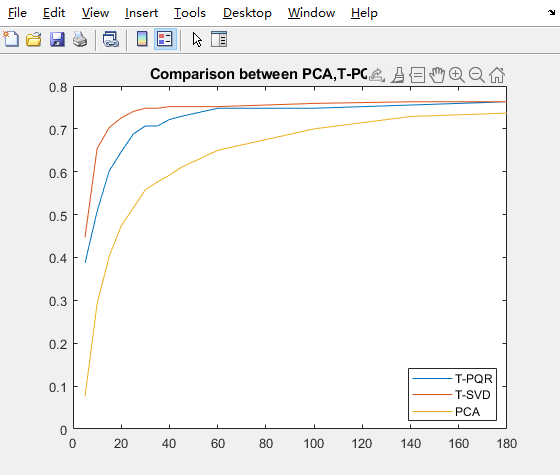
\includegraphics[scale=0.6]{all}
	\caption{Ratio Curves for Different Methods}
\end{figure}
We apply Tensor Robust PCA method in T-SVD method. The tensor can be decomposed as a combination of a tensor with $rank=171$ and a sparse tensor. Then we set $k=rank=171$ in the T-SVD method, and the ratio is 0.7632.
\subsection{Storage Comparison}
\begin{align*}
\text{Storage}_{T-SVD} = K_{T-SVD} \times  l + K_{T-SVD} \times (\text{num of training images})\\
\text{Storage}_{T-PQR} = K_{T-PQR} \times  l + K_{T-PQR} \times (\text{num of training images})\\
\text{Storage}_{PCA} = K_{PCA} \times  l \times n + K_{PCA} \times (\text{num of training images})
\end{align*}
We compare the storage for same $k$ for different algorithms
\begin{table}[H]
	\centering
	\begin{tabular}{llll}
		\hline
		PCA & T-SVD & T-PQR & TRSVD \\
		\hline
		12.5   & 1  & 1.12  & 2.1
	\end{tabular}
\end{table}


\subsection{Time Comparison}
We compare the running time for same $k$ of different algorithms
\begin{table}[H]
	\centering
	\begin{tabular}{llll}
		\hline
		PCA & T-SVD & T-PQR & TRSVD \\
		\hline
		1   & 5.26  & 5.31  & 10.1 
	\end{tabular}
\end{table}

\subsection{Acceleration TIPS}
Use LEMMA2 to accelerate our algorithm. Time of different algorithms:
\begin{table}[H]
	\centering
	\begin{tabular}{ll}
		\hline
		T-SVD & T-SVD-With LEMMA2\\
		\hline
		9.8   & 1  
	\end{tabular}
\end{table}
\newpage
% bibliography
\nocite{*}
\bibliographystyle{plain}
\bibliography{mybib}


\end{document}